El radio del cilindro de un carrete mide 2.0 cm. Una persona, en 10 s, desenrrolla uniformemente 50 cm del hilo que está en contacto con el cilindro (véase Figura de este problema).
\begin{enumerate}
    \item ¿Cuál es el valor de la velocidad lineal de un punto de la superficie del cilindro?
    \item ¿Cuál es la velocidad angular del punto $P$, mostrado en la figura, situado a 4.0 cm del eje de rotación?
\end{enumerate}
\begin{figure}[htb]
  %\centering
  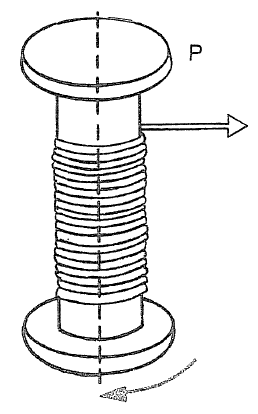
\includegraphics[scale=0.3]{figuras/fig_alvarenga_p141_17.png}
  \caption{Problema 4}
\end{figure}